\documentclass[twoside,12pt]{article}
\usepackage[left=1in, right=1in, top=1in, bottom=1in]{geometry}
\usepackage{amsmath}
\usepackage{amssymb}
\usepackage{amsfonts}
\usepackage{mathtools}
\usepackage{amsthm}
\usepackage{fancyhdr}
\usepackage{enumitem}
\usepackage{siunitx}
\usepackage{booktabs}
\usepackage[hidelinks]{hyperref}
\usepackage{sectsty}
\usepackage{mathrsfs} % mathscr
\usepackage{tikz}
\usepackage{pgfplots}
\usepackage{multicol}
\usepackage{listings}
% \usepackage{amsart}
\usepackage{fontspec}
\usepackage{titlesec}
\usepackage{subcaption}

% less hyphens, similar to tolerance?
\usepackage{microtype}

% allow H option of figure
\usepackage{float}

% math font (libertine)
\usepackage{libertinus-otf}

% braket
\usepackage{braket}

% mono font
\usepackage{inconsolata}
\setmonofont{inconsolata}

% SI units
\usepackage{siunitx}

% define Latin modern font environment
\newcommand{\lms}{\fontfamily{lmss}\selectfont} % Latin Modern Roman
% \newcommand{\lmss}{\fontfamily{lmss}\selectfont} % Latin Modern Sans
% \newcommand{\lmss}{\fontfamily{lmtt}\selectfont} % Latin Modern Mono

% % change mathcal shape
% \usepackage[mathcal]{eucal}


% define math operators
\newcommand{\FF}{\mathbb{F}}
\newcommand{\RR}{\mathbb{R}}
\newcommand{\NN}{\mathbb{N}}
\newcommand{\ZZ}{\mathbb{Z}}
\newcommand{\QQ}{\mathbb{Q}}
\newcommand{\XX}{\mathbb{Y}}
\newcommand{\CL}{\mathcal{L}}
% \renewcommand{\d}{\mathrm{d}}
\renewcommand*\d{\mathop{}\!\mathrm{d}}
\DeclareMathOperator*{\argmax}{arg\,max}
\DeclareMathOperator*{\argmin}{arg\,min}
\DeclareMathOperator{\im}{im}
\DeclareMathOperator{\id}{id}
\renewcommand{\mod}[1]{\ (\mathrm{mod}\ #1)}

% section font style
\sectionfont{\lms\large}
\subsectionfont{\lms\normalsize}
\subsubsectionfont{\bf}

% line spreading and break
\hyphenpenalty=5000
\tolerance=20
\setlength{\parindent}{0em}
\setlength\parskip{0.5em}
\allowdisplaybreaks
\linespread{0.9}

% theorem
% latex theorem
% definition style
\theoremstyle{definition}
\newtheorem{theorem}{Theorem}[subsection]
\newtheorem{axiom}{Axiom}[section]
\newtheorem{definition}{Definition}[section]
\newtheorem{example}{Example}[section]
\newtheorem{question}{Question}[section]
\newtheorem{exercise}{Exercise}[section]
\newtheorem*{exercise*}{Exercise}
\newtheorem{lemma}{Lemma}[section]
\newtheorem{proposition}{Proposition}[section]
\newtheorem{corollary}{Corollary}[section]
\newtheorem*{theorem*}{Theorem}
\newtheorem{problem}{Problem}
% remark style
\theoremstyle{remark}
\newtheorem*{remark}{Remark}
\newtheorem*{solution}{Solution}
\newtheorem*{claim}{Claim}


% paragraph indent
\setlength{\parindent}{0em}
\setlength\parskip{0.5em}

\newcommand\Code{CSC4005 FA22}
\newcommand\Ass{HW04}
\newcommand\name{Haoran Sun}
\newcommand\mail{haoransun@link.cuhk.edu.cn}

\title{{\lms \Code \ \Ass}}
\author{\lms \name \ (\href{mailto:\mail}{\mail})}
\date{\sffamily \today}

\makeatletter
% \let\Title\@title
\let\theauthor\@author
\let\thedate\@date

\fancypagestyle{plain}{%
    \fancyhf{}
    \lhead{\sffamily \Ass}
    \rhead{\sffamily \name}
    \rfoot{\sffamily\thepage}

    % # 页脚自定义
    \fancyfoot[L]{
        \begin{minipage}[c]{0.06\textwidth}
            
\includegraphics[height=7.5mm]{logo2.png}
        \end{minipage}
    }
}
\fancypagestyle{title}{%
    \fancyhf{}
    \renewcommand{\headrulewidth}{0pt}
    % \lhead{\Title}
    % \rhead{\theauthor}
    \rfoot{\sffamily\thepage}

    % # 页脚自定义
    \fancyfoot[L]{
        \begin{minipage}[c]{0.06\textwidth}
            
\includegraphics[height=7.5mm]{logo2.png}
        \end{minipage}
    }
}
\fancyfootoffset[L]{0.3cm}

% re-define title format
% \makeatletter
% \renewcommand{\maketitle}{\bgroup\setlength{\parindent}{0pt}
% \begin{flushleft}
%   \textbf{\Large\@title}
%   \@author
% \end{flushleft}\egroup
% }
% \makeatother
\makeatletter
\renewcommand{\maketitle}{\bgroup\setlength{\parindent}{0pt}
\begin{center}
  \textbf{\Large\@title}\\
  \@author
\end{center}\egroup
}
\makeatother

\pagestyle{plain}

% lstlisting settings
\lstset{
    basicstyle=\linespread{0.8}\ttfamily\small,
    breaklines=true,
    basewidth=0.5em,
    frame=single,
}
\lstdefinestyle{output}{
    basicstyle=\linespread{0.8}\ttfamily\footnotesize,
    breaklines=true,
    basewidth=0.5em,
    frame=single,
}    
\lstdefinestyle{sh}{
    basicstyle=\linespread{0.8}\ttfamily\footnotesize,
}
\lstdefinestyle{cpp}{
    numbers=left,
    basicstyle=\linespread{0.8}\ttfamily\footnotesize,
    numberstyle=\linespread{0.8}\ttfamily\footnotesize,
    language=C++,
    xleftmargin=6.0ex,
    frame=single,
}


\begin{document}
\begin{titlepage}
    \maketitle
    \thispagestyle{title}
\end{titlepage}

\section{Introduction}
In this project, a heat distribution model using Jacob iteration (same as finite difference)
is implemented.
Despite a sequential version, the program is also accelerated by
common parallelization libraries: MPICH, OpenMP, Pthread, and CUDA.
The performance of each method is evaluated.




\section{Method}
\subsection{System setup}
The system contains a $n\times n$ square 2D mesh 
with temperature assigned
where $x$ ranging in $[-5,5]$ and $y$ ranging in $[-5,5]$.
Initially, fire regions $\Omega$ is defined as $\{(x,y)|x^2+y^2\leq 1\}$,
and temperature will be assigned to \SI{100}{\celsius}.
Other region will be assigned to \SI{20}{\celsius}.
Note that all fire regions will keep \SI{100}{\celsius}
and all boundary (edge) region $\{(x,y)|x=--5,5; y=-5,5\}$
will keep \SI{100}{\celsius}.


\subsection{Program design and implementation}
The programs are written in the C++ programming language.
MPICH, Pthread, OpenMP, and CUDA libraries were used for parallelization.
Besides, OpenGL is used for visualization purposes.
Also, to improve the performance, the MPI version is further accelerated
using OpenMP.

Despite MPI version written separately in \lstinline|src/main.mpi.cpp|, 
the main program of other version are all wrapped
in \lstinline|src/main.cpp|.
Particularly, CUDA functions are compiled in a separated library
\lstinline|build/lib/libcudalib.a|.

One can refer to \ref{fig:flowchart} to understand the program design.


\subsection{Usage}
\begin{remark}
For convenience, one can directly build the program by \lstinline|scripts/build.sh|
to compile all targets.
\end{remark}
To simplify the compiling process, the CMake build system is used
to compile programs and link libraries.
One can execute the following lines to build executables.
\begin{lstlisting}[style=sh]
cmake -B build -DCMAKE_BUILD_TYPE=Release -DGUI=ON
cmake --build build
\end{lstlisting}
To disable the GUI feature, one can set \lstinline|-DGUI=OFF| in the first line.
The compiled programs and libraries are shown in the \lstinline|build/bin| and
\lstinline|build/lib|.
One can directly execute \lstinline|build/bin/main*.gui| for a visualized demonstration.
\begin{lstlisting}[style=sh]
./build/bin/main.seq.gui
./build/bin/main.omp.gui
./build/bin/main.pth.gui
./build/bin/main.mpi.gui
./build/bin/main.cu.gui
\end{lstlisting}

One can customize the running parameters such as the number of particles $n$ and
simulation steps according to the following lines.
\begin{lstlisting}[style=sh]
./build/bin/main.seq               --dim 100 --nsteps 10000 --record 1
./build/bin/main.omp        -nt 10 --dim 100 --nsteps 10000 --record 1
./build/bin/main.omp        -nt 10 --dim 100 --nsteps 10000 --record 1
./build/bin/main.cu                --dim 100 --nsteps 10000 --record 1
mpirun -np 10 ./build/bin/main.mpi --dim 100 --nsteps 10000 --record 1
\end{lstlisting}
\begin{remark}
To execute \textbf{MPI + OpenMP} hybrid program, one can just append \lstinline|-nt [n]| parameters
when executing the MPI program.
For example, the following line initializes a program with 10 MPI process,
and each process has 2 OpenMP threads, which have $10\times 2=20$ threads in total.
\begin{lstlisting}[style=sh]
mpirun -np 10 ./build/bin/main.mpi -nt 2
\end{lstlisting}
\end{remark}


\subsection{Performance evaluation}
The program was executed under 
different configurations to evaluate performance.
With 40 different CPU core numbers (from 1 to 40 with increment 1, $p=1, 2,\dots, 40$)
and 40 different $n$ (from 50 to 2000 with increment 50),
1600 cases in total were sampled for sequential, MPI, OpenMP, and Pthread programs.
Test for CUDA program is implemented separately.
Recorded runtime is analyzed through the Numpy
package in Python.
Figures were plotted through the Matplotlib and the Seaborn packages in Python.
Analysis codes were written in \lstinline|analysis/main.ipynb|.

\begin{figure}[h!]
    \centering
    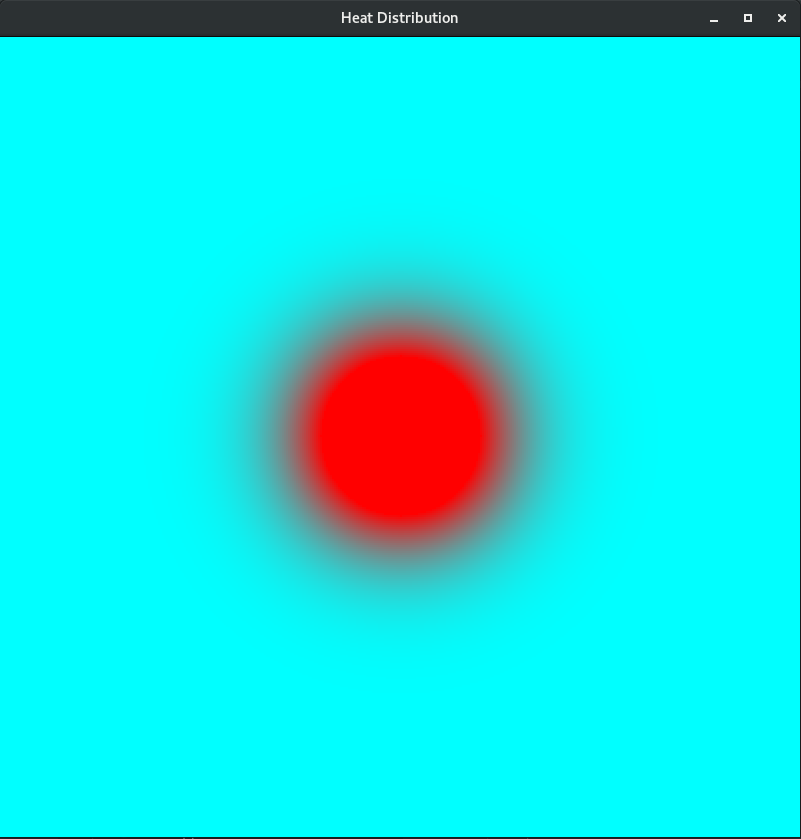
\includegraphics[width=0.5\textwidth]{../demo.png}
    \caption{Sample GUI window}
    \label{fig:image}
\end{figure}


\newpage
\section{Result and discussion}

\subsection{CPU parallelization}
From Figure \ref{fig:fps-core-cpu}, we can know that
when $n$ ranging from $1000$ to $2000$,
MPI, OpenMP, and Pthread have very different performance.
For MPI program, the fps almost monotonically decreases with the increase of overall
processes.
The reason may caused from the communication time.
It seems that the time cost of communication increase faster than
the computation time when when $n$ increase.
For OpenMP program, the fps increases linearly.
This proves that multi-thread indeed improve the performance.
For Pthread program, the fps increases with the number of threads
until it reaches it maximum when the number of threads are around $15$.

The heatmap which indicate the rate of acceleration plotted in the Figure \ref{fig:heatmap-rate-cpu} 
provides some direct visualization of the performances of parallel variants.
From this figure we can clearly know that MPI scheme has worst performance--it
is even slower when overall threads is greater than $1$.
For Pthread, we can see it reaches its maximum speed-up rate when
the number of thread is around 15.
For OpenMP program, when $n$ is large ($\geq 1400$), speed-up rate will
be higher when the number of threads is greater.

\subsection{GPU parallelization}
GPU parallelization is much more massive than CPU parallelization.
This allows one to implemented $n>10^4$ with high fps, as Figure \ref{fig:fps-dim-gpu}
shows.
Notably, the gpu shared memory is used to accelerate the read operations.
(please refer to \lstinline|__shared__| type and \lstinline|__syncthreads| function
in \lstinline|cudalib.cu|).
According to NVIDIA, the memory access on shared memory is
approximately 100$\times$ faster than the GPU memory(\lstinline|__device__|) access.

For example, a naive vector addition in CUDA could be written as
\begin{lstlisting}[style=cpp]
__global__ void VecAdd(int *a, int *b, int *c, long int dim){
    // thread partition
    int start_idx = dim / (blockDim.x * gridDim.x) * threadIdx.x;
    int end_idx   = dim / (blockDim.x * gridDim.x) * (threadIdx.x+1);
    if (threadIdx.x+1==blockDim.x) end_idx = dim;
    // vector add
    for (int i = 0; i < dim; i++){
        c[i] = a[i] + b[i];
    }
}
\end{lstlisting}
During the calculation, each thread in GPU will require to
access the memory independently.
When the overall thread number is large, the memory miss could
cost a huge amount of time.
However, in CUDA, we can split those threads into different blocks:
for example, if one call a kernel function \lstinline|kernel|
by \lstinline|kernel<<<16,64>>>()|, then he is asking CUDA
to generate 16 blocks where each block has 64 threads, overall 
$16\times 64=1024$ threads.
Similarly, \lstinline|kernel<<<1,1024>>>()| also calls the function
with 1024 threads.
In principle, \lstinline|VecAdd<<<16,64>>>(a, b, c, dim)| and
\lstinline|VecAdd<<<1,1024>>>(a, b, c, dim)| has no difference.
Now consider, if we can let threads in each block, share a 
part of memory, then can it reduce the time cost by memory miss?
Have a look at the following function
\begin{lstlisting}[style=cpp]
#define BLOCKSIZE 64
__global__ void sharedMemVecAdd(int *a, int *b, int *c, long int dim){
    // block partition
    int block_start_idx  = dim / gridDim.x * blockIdx.x;
    int block_end_idx    = dim / gridDim.x * (blockIdx.x + 1);
    if (blockIdx.x+1==gridDim.x) block_end_idx = dim;
    int total_task       = block_end_idx - block_start_idx;
    // shared memory partition
    int num_iter = (total_task + BLOCK_SIZE - 1) / BLOCK_SIZE;
    // block-wise shared memory
    __shared__ int a_t[BLOCK_SIZE*2];
    __shared__ int b_t[BLOCK_SIZE];
    __shared__ int c_t[BLOCK_SIZE];
    __syncthreads();

    // main program
    for (int i = 0; i < num_iter; i++){
    if (threadIdx.x+i*BLOCK_SIZE < block_end_idx){
        // thread
        // copy data
        a_t[threadIdx.x] = a[block_start_idx + threadIdx.x + BLOCK_SIZE*i];
        b_t[threadIdx.x] = b[block_start_idx + threadIdx.x + BLOCK_SIZE*i];
        __syncthreads();

        // vector add
        c_t[threadIdx.x] = a_t[threadIdx.x] + b_t[threadIdx.x];


        // copy data back
        c[block_start_idx + threadIdx.x + BLOCK_SIZE*i] = c_t[threadIdx.x];
        __syncthreads();
    }}
}
\end{lstlisting}
One should convince himself that \lstinline|sharedMemVecAdd<<<16,BLOCKSIZE>>>(a, b, c, dim)|
do the exact same work as \lstinline|VecAdd|.
So what is the difference here?
In each block, CUDA will create a shared memory, that is a fast memory accessible
by ALL threads within this block.
During the computation, the block will first read a memory block,
then perform computation; after all threads finish the computation,
the threads will write data back to the global memory.


\section{Conclusion}
In conclusion, four parallel computing schemes for $n$-body simulation 
are implemented and their performances are evaluated.
For large, ignoring the precision, one may use GPU to accelerate
the calculation.


\appendix
% \renewcommand\thefigure{\thesection.\arabic{figure}}
\counterwithin{figure}{section}

\newpage
\section{Supplementary figures}

\begin{figure}[h!]
    \centering
    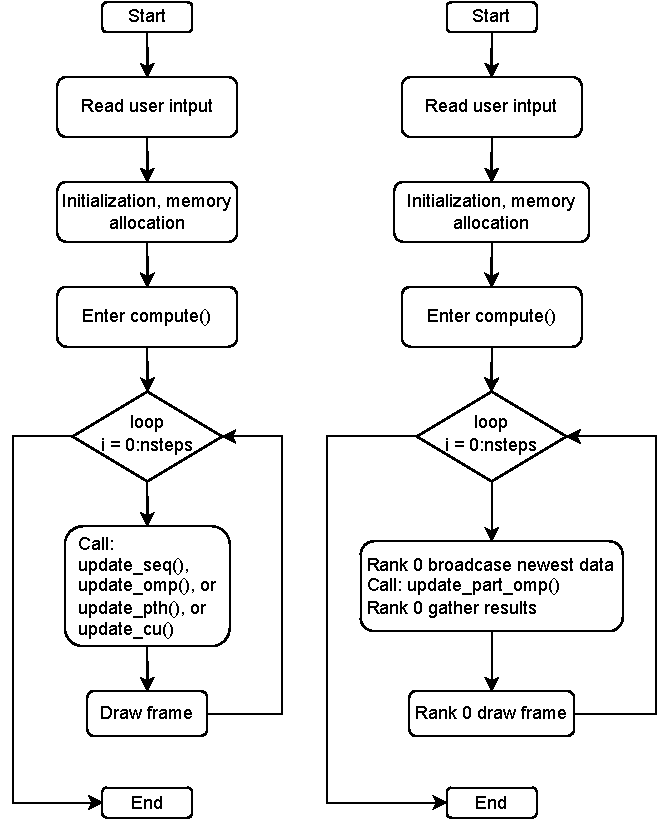
\includegraphics[width=0.95\textwidth]{../flowchart.drawio.pdf}
    \caption{Program flowchart}
    \label{fig:flowchart}
\end{figure}


\begin{figure}[h!]
    \centering
    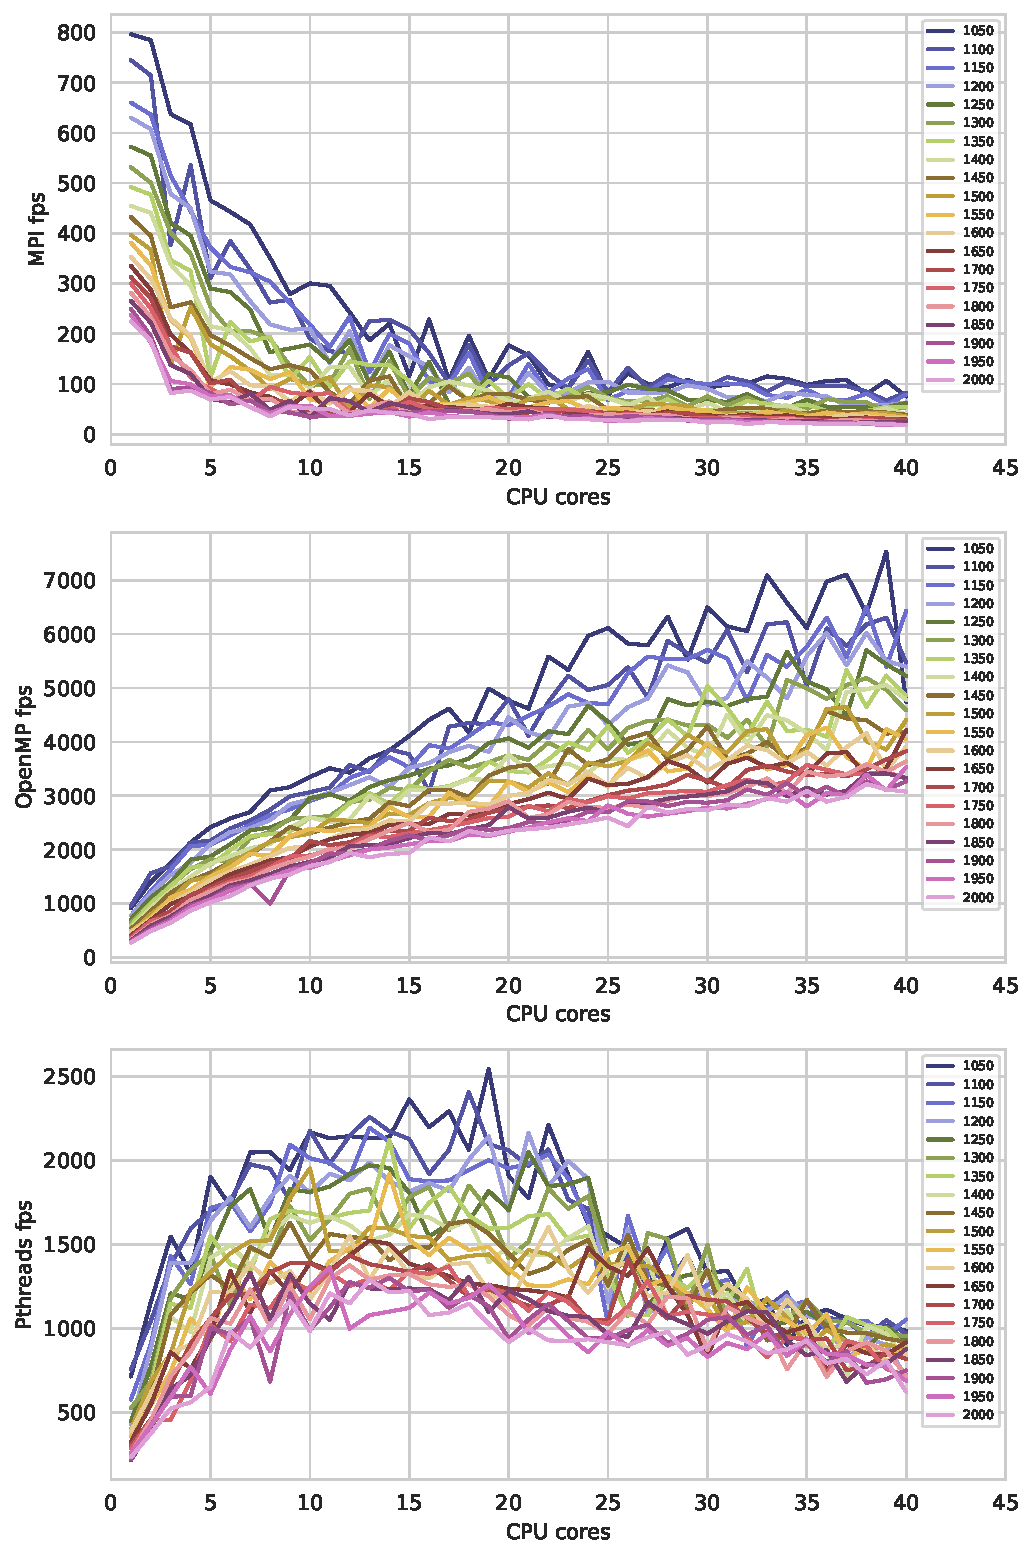
\includegraphics[height=0.95\textheight]{../analysis/fps-core-cpu.pdf}
    \caption{fps vs the number of threads/processes plot.}
    \label{fig:fps-core-cpu}
\end{figure}

\begin{figure}[h!]
    \centering
    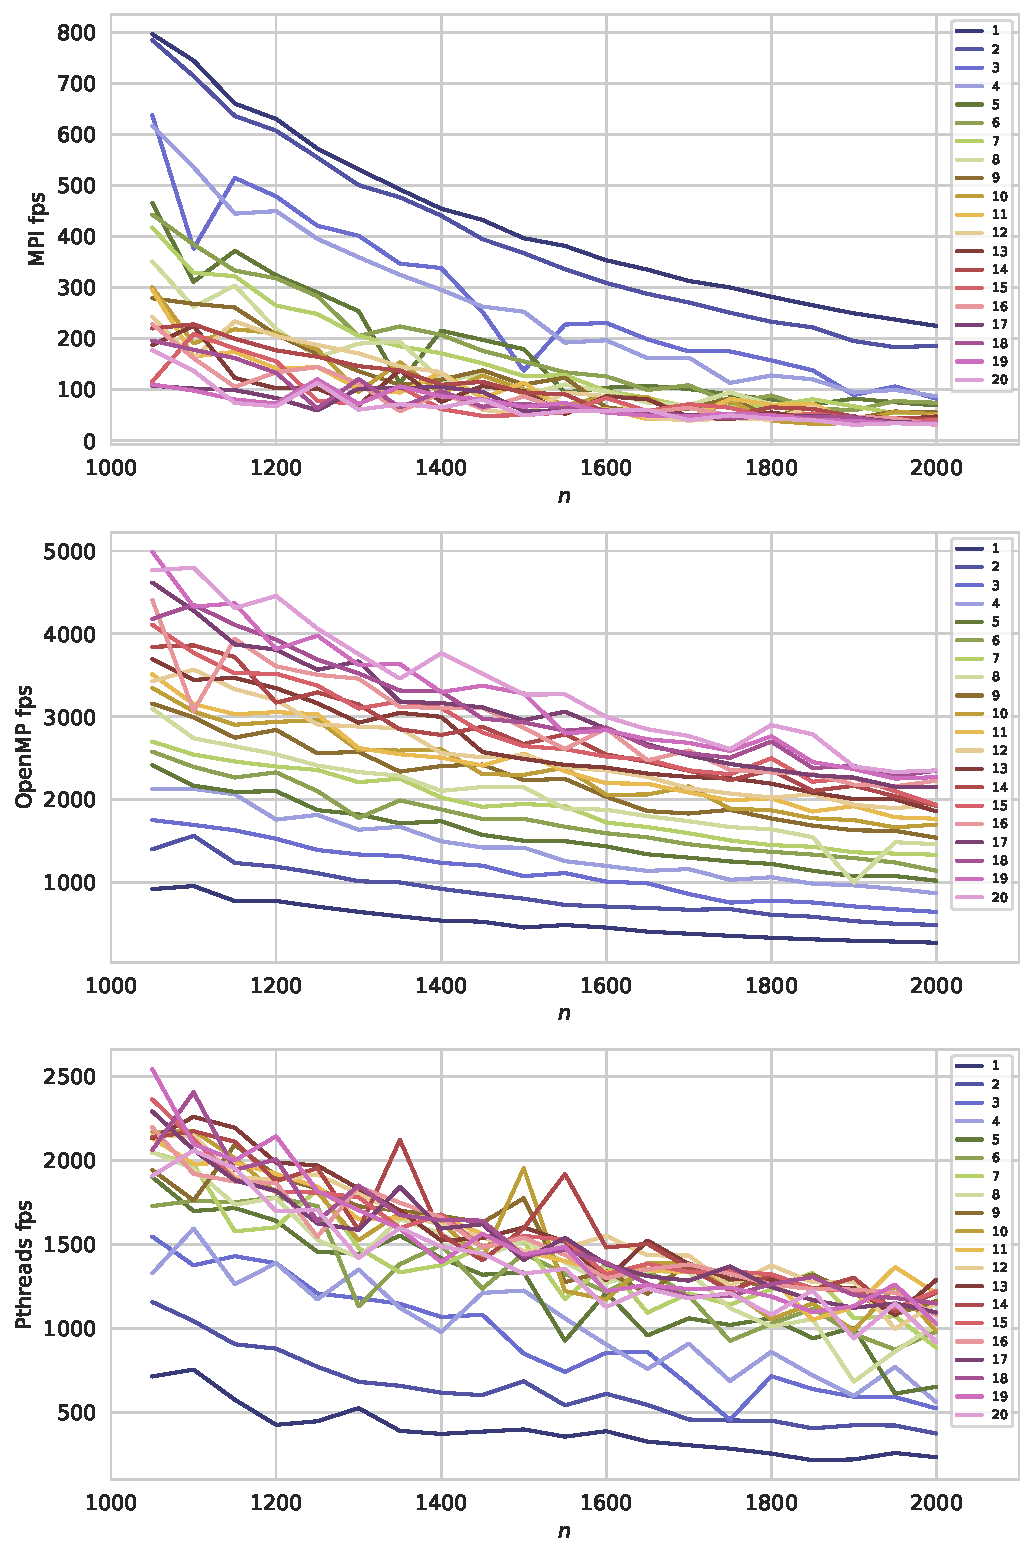
\includegraphics[height=0.95\textheight]{../analysis/fps-dim-cpu.pdf}
    \caption{fps vs the number of threads/processes plot.}
    \label{fig:fps-dim-cpu}
\end{figure}

\begin{figure}[h!]
    \centering
    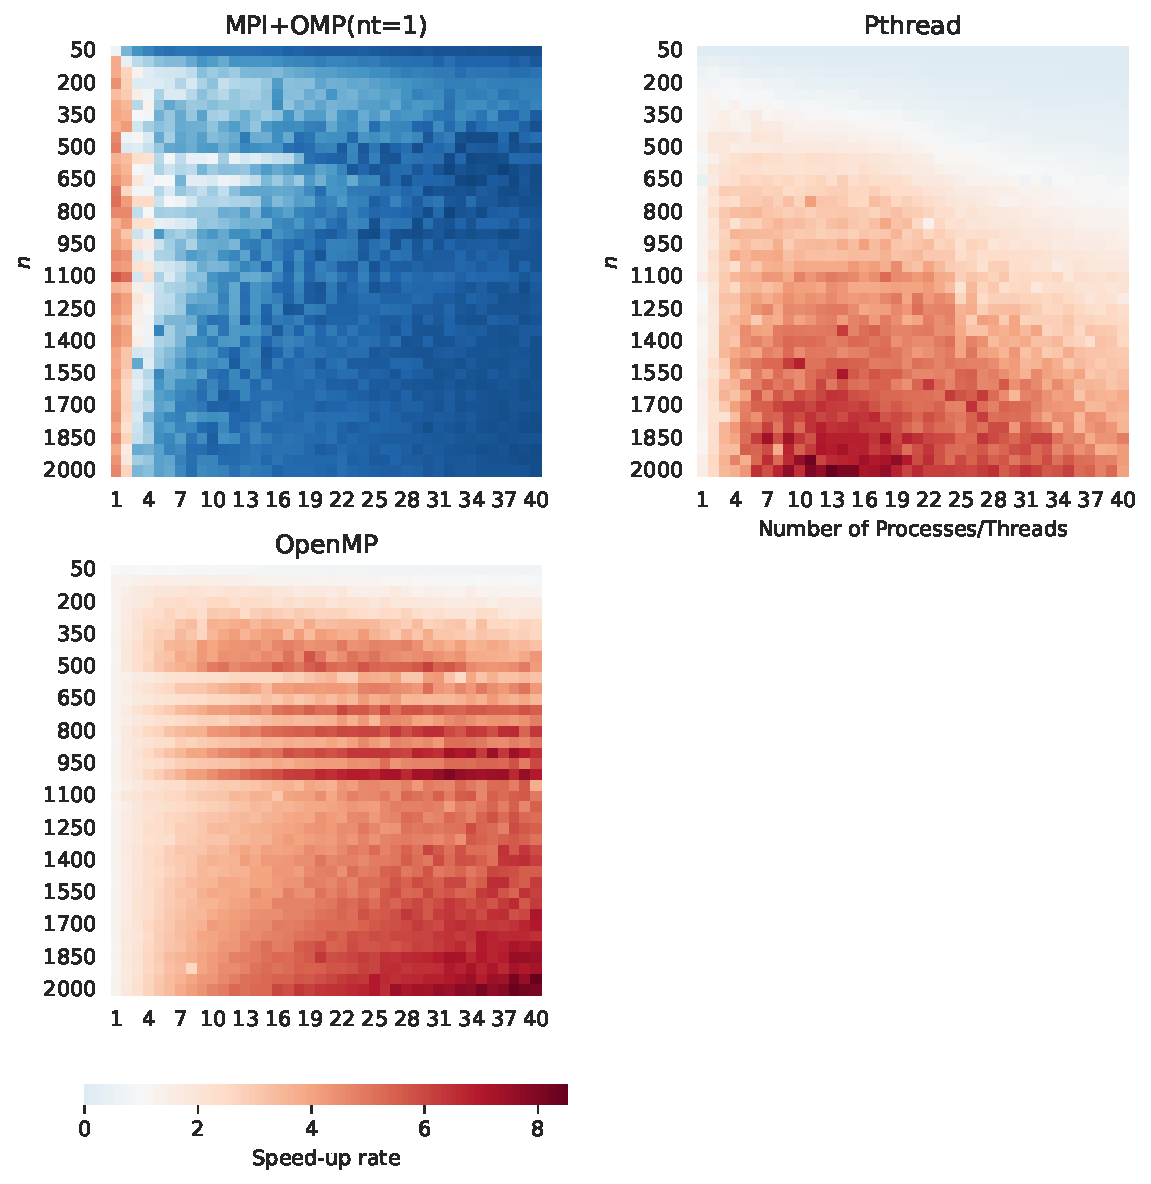
\includegraphics[width=\textwidth]{../analysis/heatmap-rate-cpu.pdf}
    \caption{Speed-up rate for multi-process/thread schemes.}
    \label{fig:heatmap-rate-cpu}
\end{figure}


\begin{figure}[t!]
    \centering
    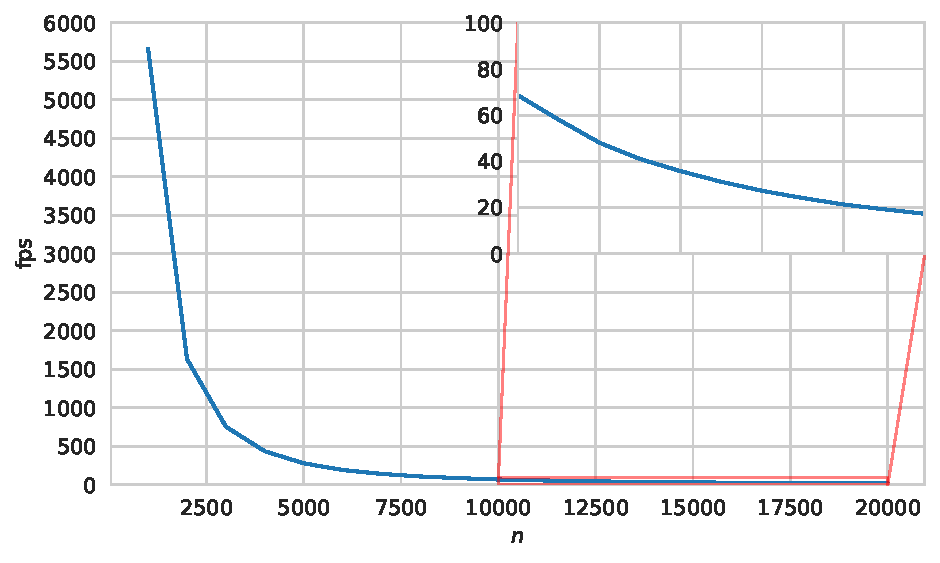
\includegraphics[width=\textwidth]{../analysis/fps-dim-gpu.pdf}
    \caption{CUDA fps vs $n$ plot.}
    \label{fig:fps-dim-gpu}
\end{figure}



\clearpage
\newpage
\section{Source code}
\lstinputlisting[style=cpp,language=,title=\lstinline|CMakeLists.txt|]{../CMakeLists.txt}
\lstinputlisting[style=cpp,language=,title=\lstinline|src/CMakeLists.txt|]{../src/CMakeLists.txt}
\lstinputlisting[style=cpp,title=\lstinline|src/main.cpp|]{../src/main.cpp}
\lstinputlisting[style=cpp,title=\lstinline|src/main.mpi.cpp|]{../src/main.mpi.cpp}
\lstinputlisting[style=cpp,title=\lstinline|src/cudalib.cu|]{../src/cudalib.cu}
\lstinputlisting[style=cpp,title=\lstinline|src/utils.h|]{../src/utils.h}
\lstinputlisting[style=cpp,title=\lstinline|src/utils.cuh|]{../src/utils.cuh}
\lstinputlisting[style=cpp,title=\lstinline|src/const.h|]{../src/const.h}




% \end{multicols*}
\end{document}

